\subsection{Ранговая селекция}\label{SetOfOperatorsAlgorithms:RankSelection}

Идентификатор: \textbf{RankSelection}.

Работает не  с массивом пригодностей напрямую, а массивом нормированных рангов, присваиваемых индивидам на основе значений пригодности. Используется функция, которая проставляет ранги для элементов несортированного массива пригодностей, то есть номера, начиная с $ 1 $, в отсортированном массиве. Если в массиве есть несколько одинаковых элементов, то ранги им присуждаются как среднеарифметические ранги этих элементов в отсортированном массиве. Если это не сделать, то вероятность выбора индивидов одинаковых по функции пригодности будет не равна друг другу, что противоречит идеи оператора селекции. Далее для выбора индивидов используется пропорциональная селекция, работающая с массивом рангов.

Значит, ранговая селекция определяется формулой:

\begin{equation}
\label{SetOfOperatorsAlgorithms:eq:RankSelection}
Selection\left( Population, Fitness, DataOfSel\right) = Random\left( \left\lbrace\bar{x}^i | p^i \right\rbrace \right),
\end{equation}
\begin{equation}
p^i=\dfrac{Rank\left( f_{fit}\left( \bar{x}^i\right)\right)  }{\sum_{j=1}^N{Rank\left( f_{fit}\left( \bar{x}^j\right)\right)}},
\end{equation}
\begin{equation}\label{SetOfOperatorsAlgorithms:eq:Rank}
Rank\left( f_{fit}\left( \bar{x}^i\right)\right)=\dfrac{\sum_{j=1}^{N}{NumberOfSorting\left( f_{fit}\left( \bar{x}^i\right), Fitness\right)  \cdot S\left(  f_{fit}\left( \bar{x}^i\right),  f_{fit}\left( \bar{x}^j\right)\right) }}{\sum_{j=1}^{N}{S\left(  f_{fit}\left( \bar{x}^i\right),  f_{fit}\left( \bar{x}^j\right)\right) }},
\end{equation}
\begin{equation}
S\left(  f_{fit}\left( \bar{x}^i\right),  f_{fit}\left( \bar{x}^j\right)\right)= \left\lbrace \begin{array}{l}
1 \text{, если } f_{fit}\left( \bar{x}^i\right)=  f_{fit}\left( \bar{x}^j\right);\\ 0\text{, если } f_{fit}\left( \bar{x}^i\right)\neq  f_{fit}\left( \bar{x}^j\right).
\end{array}\right.
\end{equation}

где $ \bar{x}^i\in Population$, $i=\overline{1,N}.$

$NumberOfSorting\left( f_{fit}\left( \bar{x}^i\right), Fitness\right)$ --- функция, возвращающая номер элемента $ f_{fit}\left( \bar{x}^i\right)) $ в отсортированном массиве $ Fitness $ в порядке возрастания.

Формула (\ref{SetOfOperatorsAlgorithms:eq:Rank}) подсчитывает средние арифметические ранги при условии, что в массиве $ Fitness $  могут встречаться одинаковые элементы.

\textbf{Пример.} Пусть $ Fitness=\left\lbrace 0,5; 0,2; 0,1; 0,6; 0,2; 0,4\right\rbrace $. Тогда вероятности выбора индивидов равны:
\begin{flalign*}
p_1&=\frac{5}{5+2,5+1+6+2,5+4}=0,238;\\
p_2&=\frac{2,5}{5+2,5+1+6+2,5+4}=0,119;\\
p_3&=\frac{1}{5+2,5+1+6+2,5+4}=0,047;;\\
p_4&=\frac{6}{5+2,5+1+6+2,5+4}=0,286;\\
p_5&=\frac{2,5}{5+2,5+1+6+2,5+4}=0,119;\\
p_6&=\frac{4}{5+2,5+1+6+2,5+4}=0,190.
\end{flalign*}

\begin{figure} [H] 
  \center
  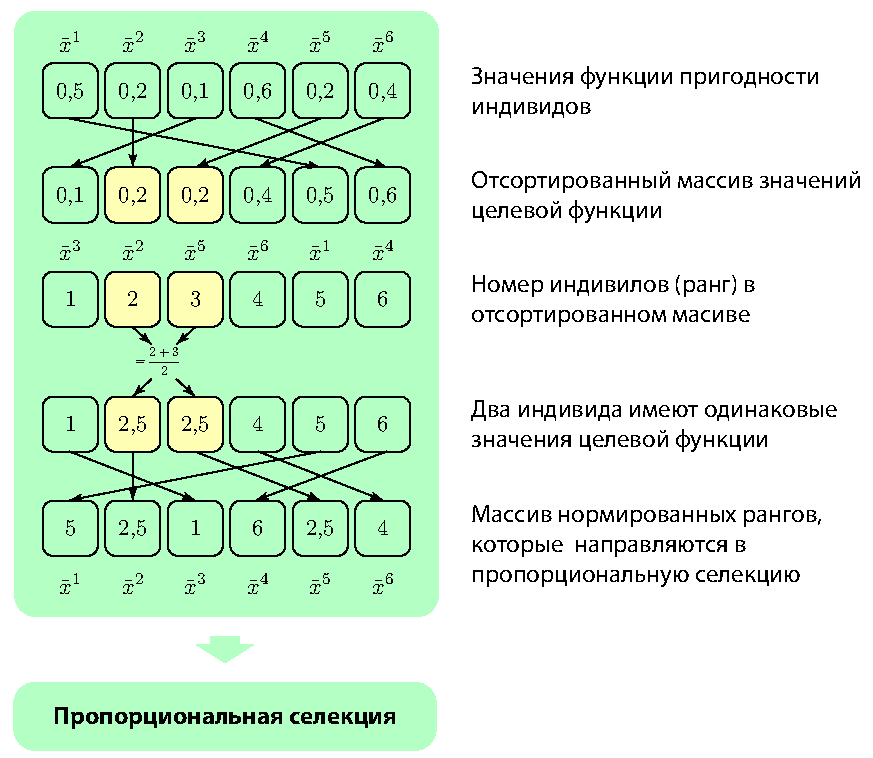
\includegraphics [scale=0.7] {RankSelection}
  \caption{Механизм работы ранговой селекции} 
  \label{SetOfOperatorsAlgorithms:img:RankSelection}  
\end{figure}

$ DataOfSel $ также не содержит каких-либо параметров относительно данного типа селекции.

Нет ограничений на множество задач оптимизации, которые может решать алгоритм оптимизации с данной селекцией.

В библиотеке \textbf{HarrixMathLibrary} данная селекция реализуется через функцию \textbf{MHL\_RankSelection}:

\href{https://github.com/Harrix/HarrixMathLibrary}{https://github.com/Harrix/HarrixMathLibrary}